\scanpage{30}
\uline{NB} Il y a a priori deux structures carrées sur $T\setminus\{\tau\}$ satisfaisant 1°), définies par les deux bijections possibles entre $\Phi\setminus\{\tau\}=\Omega'$ et $\Omega$ (relation de non-adjacence), mais on constate que les 2 \deleted{signatures} \inserted{orientations} de $T$ associées à ces deux choix de $\gamma$, lorsque $\alpha$ satisfait tjrs 2°), sont opposées, donc il y a exactemt un tel $\gamma$ tel que $(\tau,\gamma,\alpha)\in\mathbb A^+(T,\unsure{\bar\omega|\varpi})$ \ldots

\[
\bigl[\ R'=A^{\uparrow}(\bar\Pi)\simeq
\{(\Omega\unsure{'|^{\bullet}|\mbox{}},\Omega')\in\unsure{\mathscr P|\mathfrak P}_2(T)\times\mathscr P_2(T)\mid\Omega\cap\Omega'=\varnothing\}
\]

c) $\bar s$ et $\bar f$ sont incidents sss $\Omega$ est une \uline{\unsure{anticôte|anticôté}} pour la structure pentagonale $\pi$. [$R''\simeq{}$ ens des structures pentagonales sur $T$ munies d'une (anti) \unsure{côte|côté|arête} \inserted{au choix}]

\figure{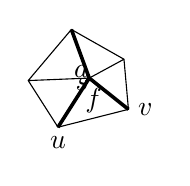
\begin{tikzpicture}[scale=.63]
\coordinate(a)at(-1,0);\coordinate(b)at(-.13,1.03);\coordinate(c)at(.93,.43);
\coordinate(d)at(1.02,-.58);\coordinate(e)at(-.40,-.94);\coordinate(s)at(.23,.05);
\draw(a)--(b)--(c)--(d)--(e)--cycle (a)--(s)--(c);
\draw[line width=1.3pt](b)--(s)--(e) (s)--(d);
\node[above left,inner sep=0pt] at (s){$a$};\node[below left,inner sep=0pt]at(s){$s$};
\node at (.32,-.40){$f$};\node[below]at(e){$u$};\node[right]at(d){$v$};
\end{tikzpicture}}
\margin{\uline{NB} $a\sim\{u,v\}$}

d) $\{\bar s,\bar a,\bar f\}$ forment un repère sss $\pi,(\tau,\gamma,\alpha)$ et $\Omega$ se déduisent de
$\{\underset{\inserted{\substack{\uparrow\\\mathrm{Pent}^+(T,\bar\omega)}}}{\pi},
\underset{\inserted{\substack{\uparrow\\T}}}{\tau},
\underset{\inserted{\substack{\uparrow\\\mathscr P_2(T)}}}{\Omega}\}$
satisfaisant $\tau\notin\Omega$, $\Omega$ anticôte pour $\pi$, $\tau$ adjacent \inserted{(pour $\pi$)} à un \uline{seul} sommet de $\Omega$
[ce qui donne, pour \deleted{\unsure{$\mathscr P_2$}} $\pi$ (6 choix) et $\Omega$ (5 \deleted{\unsure{et}} choix) choisis, 2 choix pour $\tau$], en prenant pour $\gamma$ l'unique structure de carré sur $T\setminus\{\tau\}$ pour laquelle $\Omega$, $\{u,v\}$ (ens des deux sommets adj. à $t$ \unsure{\}|)} et $\{\bar u,\bar v\}=T\setminus\{\tau\}-\{u,v\}$ sont des arêtes, et $\alpha=\{\{u,v\},\{\tilde u,\tilde v\}\}$ est le \unsure{contingent|côté-gauche|codiagonale} de $(T\setminus\{\tau\},\gamma\}$ qui ne contient pas $\Omega$. La donnée

\diagram{\begin{tikzcd}[ampersand replacement=\&,row sep=tiny,column sep=tiny]
\&\& A^{\vcenter{\hbox{\tikz[scale=.1]{\draw[->](0,0)--(0,1.5);\draw[->](0,0)--(1.5,0);}}}}\arrow[ddl]\arrow[d]\arrow[ddr]\&\&\\
\&\& A^{\wedge}\arrow[ddl]\arrow[ddr]\&\&\\
\&\vec A\arrow[dl]\arrow[dr]\&\& A^{\uparrow}\arrow[dl]\arrow[dr]\&\\
S\&\& A\&\& F
\end{tikzcd}}
\figure{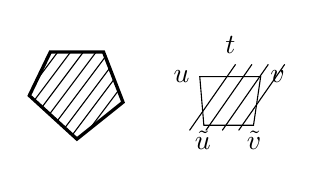
\begin{tikzpicture}[scale=.65]
\begin{scope}\clip (-.93,.05)--(-.52,.9)--(.52,.9)--(.9,-.08)--(0,-.8)--cycle;
\foreach \x in {-1.8,-1.55,...,1}{\draw (\x,-1)--++(1.5,2);}\end{scope}
\draw[very thick](-.93,.05)--(-.52,.9)--(.52,.9)--(.9,-.08)--(0,-.8)--cycle;
\begin{scope}[xshift=3cm]
\node at(0,1.03){$\deleted{\unsure{t}}$};\draw (-.6,.42)--(.59,.42)--(.45,-.53)--(-.52,-.53)--cycle;
\foreach \x in {-.8,-.48,-.16,.16}{\draw(\x,-.63)--++(.90,1.29);}
\node[left]at(-.61,.43){$\deleted{\unsure{u}}$};\node[right]at(.59,.42){$\deleted{\unsure{v}}$};
\node[below]at(-.54,-.46){$\deleted{\unsure{\tilde u}}$};\node[below]at(.46,-.46){$\deleted{\unsure{\tilde v}}$};
\end{scope}\end{tikzpicture}}
\figure{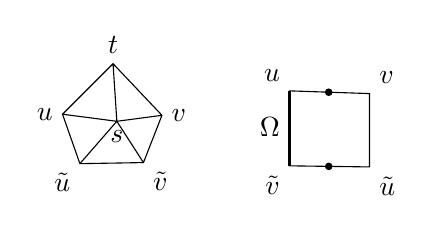
\begin{tikzpicture}[scale=.69]
\coordinate(t)at(0,1.2);\coordinate(u)at(-.93,.27);\coordinate(v)at(.90,.25);
\coordinate(x)at(-.61,-.64);\coordinate(y)at(.56,-.62);\coordinate(s)at(.07,.14);
\draw (u)--(t)--(v)--(y)--(x)--cycle (x)--(s)--(y) (u)--(s)--(v) (t)--(s);
\node[above]at(t){$t$};\node[left]at(u){$u$};\node[right]at(v){$v$};\node[below]at(s){$s$};
\node[below left]at(x){$\tilde u$};\node[below right]at(y){$\tilde v$};
\begin{scope}[xshift=4cm]
\draw(-.75,.7)--(.72,.65)--(.72,-.7)--(-.75,-.68)--cycle;
\draw[very thick](-.75,.7)--(-.75,-.68);
\fill (-.03,.675) circle(2pt) (-.03,-.69) circle(2pt);
\node[above left]at(-.75,.7){$u$};\node[above right]at(.72,.65){$v$};
\node[left]at(-.75,.04){$\Omega$};\node[below left]at(-.75,-.68){$\tilde v$};
\node[below right]at(.72,-.7){$\tilde u$};
\end{scope}\end{tikzpicture}}
% archive sheet number: 29
